\chapter{Communication}

As a rule the medium of communication for Engineers is \textit{drawings}. Engineering is a highly complex field, is information dense and difficult to transmit ideas non-visually. You can have a specification which is six pages long for an example a cooling tower. On a Drawing a simple drawing can describe all that information in a more concise and clear way.

Many other items can be described in traditional documents use in construction:

\begin{figure}
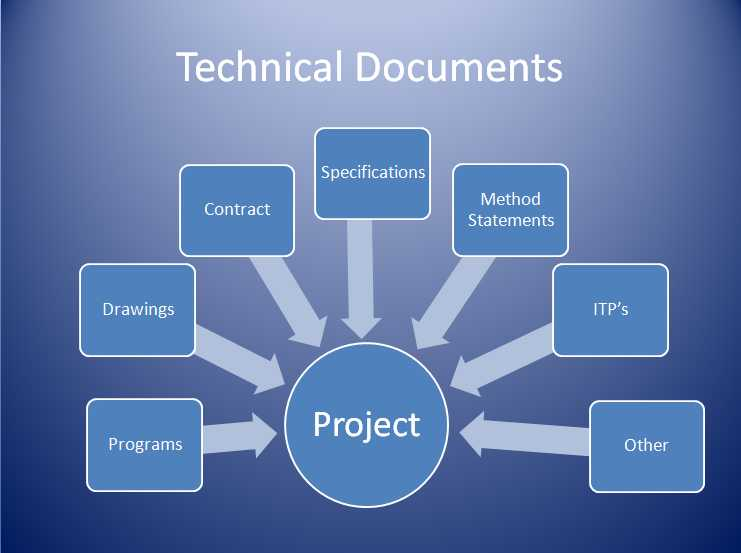
\includegraphics[width=\textwidth]{./graphics/process-02}
\end{figure}

What materials are we going to Supply? This is communicated through technical submittals.

How are we going to install them and test them? This is communicate through ITP's and Method Statements.

When are we going to carry out the work? This is communicated through a Programme of Works.

Who is doing What? This is normally through our organization charts?

Many a better head than this writers have found ways to manage projects along these documents. Although sometimes when misused can cause undue delays, the absence of them can lead to a disastrous Project.

Engineers are not good communicators in general, they work long hours and under pressure making communication more difficult. Try and put as much information on
a drawing as possible. Remember they used to be called plans.


In general we try to commuicate with documents. By utilizing documents rather than verbally communicating requests, actions and the like, documents can flow better. In general use the phone, if you can achieve what you want with the phone-call (such as obtaing the status for something). If the action you request from the person who is next on line will only be completed after a few days commuicate in writing.

\subsection*{Follow-ups}

A message flows better between two people rather than a number of persons. In designing our processes we have kept that in mind. As a rule of thumb if you need to follow-up on a particular action, you need to do it with the person you have send the document to. As an example you have send a request for a purchase. It is no good phoning the Area Manager iff he had approved it or the Financial Department if he has issued the check. You need to follow with the Department head to whom you have addressed the documents. (He might have just finished a meeting with the Financial Manager and a direct call to Accounts, in a way will relieve the MCD Department of his responsibility to expedite)!

\begin{figure}
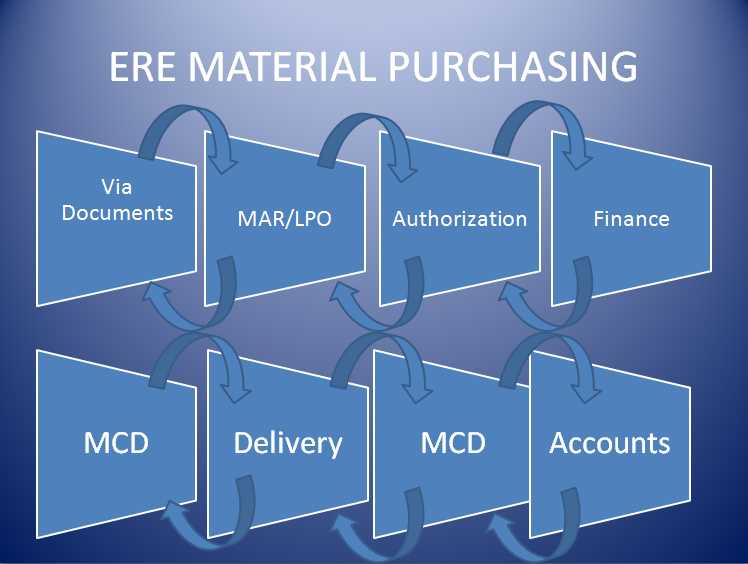
\includegraphics[width=\textwidth]{./graphics/process-01}
\end{figure}

\subsection*{External communications}

Our philosophy is to strive and be professional with our interactions with other Companies. In general we will take a non-confrontational attitude that is pro-active and logical. This does not mean however that we will not stand for our rights.

\subsection*{Documentation}

All documentation with external Companies should be in writing. Either being our own suppiers and sub-contractors or the Client and other members of the professional team. Special care should be taken in approval of variation orders, invoices and other similar issues to our sub-contractors.